\subsection{Memento (备忘录)}

\noindent\textbf{意图}

在不破坏封装性的前提下,捕捉一个对象的内部状态,并在该对象之外保存这个状态这样以后就可将该对象恢复到原先保存的状态。

别名: Token

\noindent\textbf{动机}

有时有必要保存一个对象的内部状态。为了允许用户取消不确定的操作或从错误中恢复过来,需要实现检查点和取消机制,而要实现这些机制,必须事先将状态信息保存在某处,这样才能将对象恢复到它们先前的状态。

一个备忘录(memento)是一个对象,它存储另一个对象在某个瞬间的内部状态,而后者称为备忘录的原发器。

\noindent\textbf{适用性}

\begin{itemize}
    \item 必须保存一个对象在某个时刻的(部分)状态,这样以后需要时它才能恢复到先前的状态。
    \item 如果一个接口让其他对象直接得到这些状态,将会暴露对象的实现细节并破坏对象的封装性。
\end{itemize}

\noindent\textbf{结构}

\begin{figure}[H]
    \scriptsize
    \centering
    \begin{tikzpicture}[scale = 1]
        \begin{class}[text width=3cm]{Originator}{0,0}
            \operation{SetMemento(Memento m)}
            \operation{CreateMemento}
            \attribute{state}
        \end{class}
        \begin{class}[text width=1.5cm]{Memento}{4,0}
            \attribute{state}
            \operation{GetState()}
            \operation{SetState()}
        \end{class}
        \begin{class}[text width=2cm]{Caretaker}{8,0}
        \end{class}
        \aggregation{Caretaker}{memento}{}{Memento}
        \draw[umlcd style,fill opacity=0,fill=white,->] (Originator) -- (Memento);
    \end{tikzpicture}
\end{figure}

\noindent\textbf{参与者}

\begin{itemize}
    \item \textbf{Memento}: 存储原发器对象的内部状态。原发起根据需要决定备忘录存放原发器的哪些内部状态;防止原发器以外的其他对象访问备忘录。
    \item \textbf{Originator}: 原发器创建一个备忘录,用以记录当前时刻它的内部状态;使用备忘录恢复内部状态。
    \item \textbf{Caretaker}: 负责保存好备忘录;不能对备忘录的内容进行操作或检查。
\end{itemize}

\noindent\textbf{协作}

\begin{itemize}
    \item 管理者向原发器请求一个备忘录,保存一段时间后,将其送回给原发器,如下面的交互图所示:
    \item 备忘录是被动的。只有创建备忘录的原发器会对它的状态进行赋值和检索。
\end{itemize}

\begin{figure}[H] 
    \centering 
    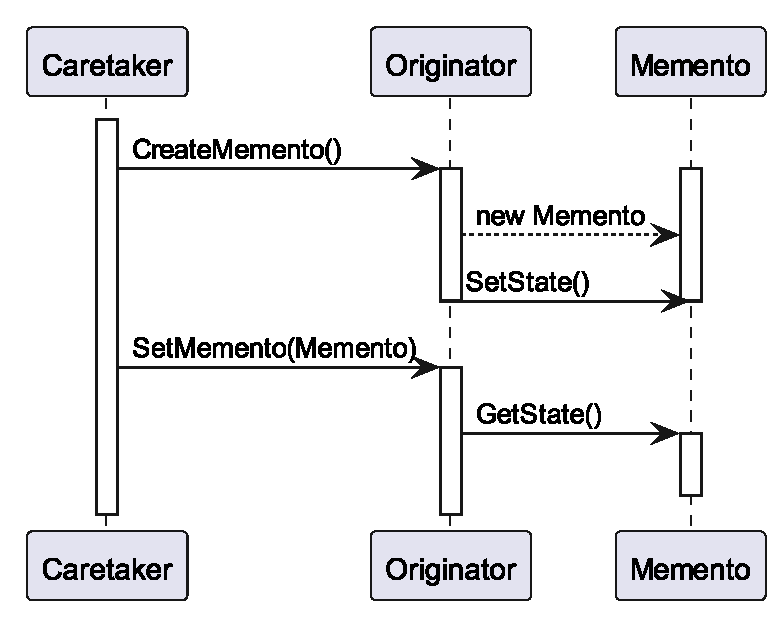
\includegraphics[width=8cm]{figures/Memento.eps} 
\end{figure}

\noindent\textbf{优缺点}

\begin{itemize}
    \item \textbf{保持封装边界}: 使用备忘录可以避免暴露一些只应由原发器管理却又必须存储在原发器之外的信息。
    \item \textbf{使用备忘录可能代价很高}: 如果用户频繁地创建备忘录和恢复原发器状态,且需要拷贝大量的信息,可能会导致非常大的开销。
    \item \textbf{维护备忘录的潜在代价}: 管理者负责删除它所维护的备忘录。然而,管理者不知道备忘录中有多少个状态。因此当存储备忘录时,一个本来很小的管理者可能会产生大量的存储开销。
\end{itemize}

\noindent\textbf{例子}

\begin{itemize}
    \item Java: \url{https://blog.csdn.net/yuanchangliang/article/details/119211105}
    \item Video: \url{https://www.bilibili.com/video/BV1Sv41167o6}
\end{itemize}

\lstinputlisting[language=Python]{../../scripts/behavioral/Memento.py}

\newpage